\subsubsection{Averaging material properties}
\label{sec:sinker-with-averaging}

\textit{The original motivation for the functionality discussed here, as well
  as the setup of the input file, were provided by Cedric Thieulot.}

Geophysical models are often characterized by abrupt and large jumps in material
properties, in particular in the viscosity. An example is a subducting, cold
slab surrounded by the hot mantle: Here, the strong
temperature-dependence of the viscosity will lead to a sudden jump in the
viscosity between mantle and slab. The length scale over which this jump happens
will be a few or a few tens of kilometers. Such length scales cannot be
adequately resolved in three-dimensional computations with typical meshes for
global computations.

Having large viscosity variations in models poses a variety of problems to
numerical computations. First, you will find that they lead to very long compute
times because our solvers and preconditioners break down. This may be
acceptable if it would at least lead to accurate solutions, but large viscosity
gradients lead also to large pressure gradients, and this in turn leads to over-
and undershoots in the numerical approximation of the gradient. We will
demonstrate both of these issues experimentally below.

One of the solution to such problems is the realization that one can mitigate
some of the effects by averaging material properties on each cell somehow
(see, for example, \cite{Bab08,Deu08,DMGT11,Thi15,TMK14}).
Before going into detail, it is important to realize that if we choose material
properties not per quadrature point when doing the integrals for forming the
finite element matrix, but per cell, then we will lose accuracy in the solution
in those cases where the solution is smooth. More specifically, we will likely
lose one or more orders of convergence. In other words, it would be a bad idea
to do this averaging unconditionally. On the other hand, if the solution has
essentially discontinuous gradients and kinks in the velocity field, then at
least at these locations we cannot expect a particularly high convergence order
anyway, and the averaging will not hurt very much either. In cases where
features of the solution that are due to strongly varying viscosities or other
parameters, dominate, we may then as well do the averaging per cell.

To support such cases, \aspect{} supports an operation where we evaluate the
material model at every quadrature point, given the temperature, pressure,
strain rate, and compositions at this point, and then either (i) use these
values, (ii) replace the values by their arithmetic average $\bar x = \frac 1N
\sum_{i=1}^N x_i$, (iii) replace the values by their harmonic average $\bar x
= \left(\frac 1N \sum_{i=1}^N \frac{1}{x_i}\right)^{-1}$, (iv) replace the
values by their geometric average $\bar x
= \left(\prod_{i=1}^N \frac{1}{x_i}\right)^{-1/N}$,
or (v) replace the
values by the largest value over all quadrature points on this cell. Option
(vi) is to project the values from the quadrature points to a bi- (in 2d) or
trilinear (in 3d) $Q_1$ finite element space on every cell, and then evaluate this
finite element representation again at the quadrature points. Unlike the other
five operations, the values we get at the quadrature points are not all the
same here.

We do this operation for all quantities that the material model computes,
i.e., in particular, the viscosity, the density, the compressibility, and the
various thermal and thermodynamic properties. In the first 4 cases, the
operation guarantees that the resulting material properties are bounded below
and above by the minimum and maximum of the original data set. In the last
case, the situation is a bit more complicated: The nodal values of the $Q_1$
projection are not necessarily bounded by the minimal or maximal original
values at the quadrature points, and then neither are the output values after
re-interpolation to the quadrature points. Consequently, after projection, we
limit the nodal values of the projection to the minimal and maximal original
values, and only then interpolate back to the quadrature points.

We demonstrate the effect of all of this with the ``sinker'' benchmark. This
benchmark is defined by a high-viscosity, heavy sphere at the center of a
two-dimensional box. This is achieved by defining a compositional field that is
one inside and zero outside the sphere, and assigning a compositional dependence
to the viscosity and density. We run only a single time step for this benchmark.
This is all modeled in the following input file that can also be found in
\url{cookbooks/sinker-with-averaging/sinker-with-averaging.prm}:
\lstinputlisting[language=prmfile]{full.prm.out}

The type of averaging on each cell is chosen using this part of the input file:
\lstinputlisting[language=prmfile]{harmonic.prm.out}
For the various different averaging options, and for different levels of mesh
refinement, Fig.~\ref{fig:sinker-with-averaging-pressure} shows
pressure plots that illustrate the problem with oscillations of the discrete
pressure. The important part of these plots is not that the solution looks
discontinuous -- in fact, the exact solution is discontinuous at the edge of the
circle\footnote{This is also easy to try experimentally -- use the input file
from above and select 5 global and 10 adaptive refinement steps, with the
refinement criteria set to \texttt{density}, then visualize the solution.} --
but the spikes that go far above and below the ``cliff'' in the pressure along
the edge of the circle. Without averaging, these spikes are obviously orders
of magnitude larger than the actual jump height. The spikes do not disappear
under mesh refinement nor averaging, but they become far less pronounced with
averaging. The results shown in the figure do not really allow to draw
conclusions as to which averaging approach is the best; a discussion of this
question can also be found in \cite{Bab08,Deu08,DMGT11,TMK14}).

A very pleasant side effect of averaging is that not only does the solution
become better, but it also becomes cheaper to compute.
Table~\ref{tab:sinker-with-averaging-iteration-counts} shows the
number of outer GMRES iterations when solving the Stokes
equations~\eqref{eq:stokes-1}--\eqref{eq:stokes-2}.%
\footnote{The outer iterations are only part of the problem. As discussed in
  \cite{KHB12}, each GMRES iteration requires solving a linear system with the
  elliptic operator $-\nabla \cdot 2 \eta \varepsilon(\cdot)$. For highly
  heterogeneous models, such as the one discussed in the current section, this
  may require a lot of Conjugate Gradient iterations. For example, for 8
  global refinement steps, the 30+188 outer iterations without averaging shown
  in Table~\ref{tab:sinker-with-averaging-iteration-counts} require a total of
  22,096 inner CG iterations for the elliptic block (and a total of 837 for the
  approximate Schur complement). Using harmonic averaging, the 30+26 outer
  iterations require only 1258 iterations on the elliptic block (and 84 on the
  Schur complement). In other words, the number of inner iterations per outer
  iteration (taking into account the split into ``cheap'' and ``expensive''
  outer iterations, see \cite{KHB12}) is reduced from 117 to 47 for the
  elliptic block and from 3.8 to 1.5 for the Schur complement.}
The implication of these results is that the averaging gives us a solution
that not only reduces the degree of pressure over- and undershoots, but is also
significantly faster to compute: for example, the total run time for 8 global
refinement steps is reduced from 5,250s for no averaging to 358s for harmonic
averaging.


\begin{figure}[htb]
  \centering
  \begin{tabular}{cccccc}
    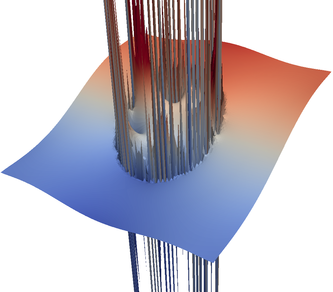
\includegraphics[width=0.14\textwidth]{q2q1/sinker-7-none.png}
    &
    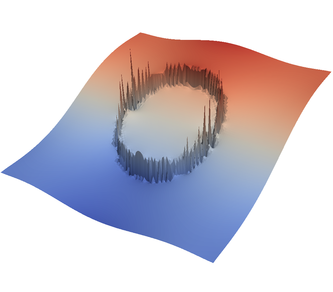
\includegraphics[width=0.14\textwidth]{q2q1/sinker-7-arithmetic.png}
    &
    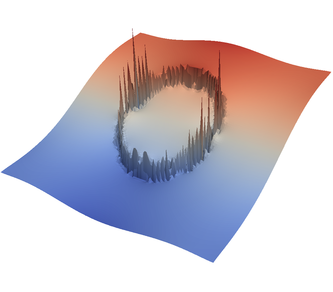
\includegraphics[width=0.14\textwidth]{q2q1/sinker-7-harmonic.png}
    &
    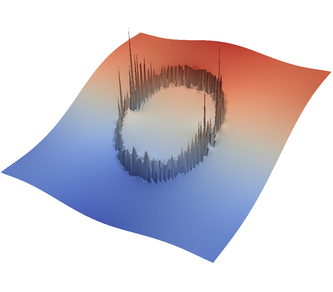
\includegraphics[width=0.14\textwidth]{q2q1/sinker-7-geometric.png}
    &
    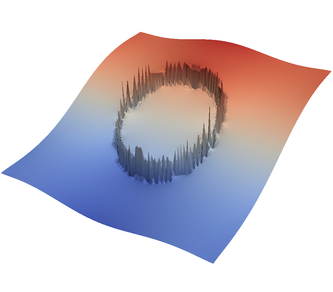
\includegraphics[width=0.14\textwidth]{q2q1/sinker-7-largest.png}
    &
    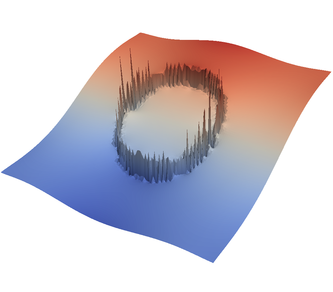
\includegraphics[width=0.14\textwidth]{q2q1/sinker-7-project.png}
    \\
    $[-45.2,45.2]$
    &
    $[-2.67,2.67]$
    &
    $[-3.58,3.58]$
    &
    $[-3.57,3.57]$
    &
    $[-1.80,1.80]$
    &
    $[-2.77,2.77]$
    \\
    \\
    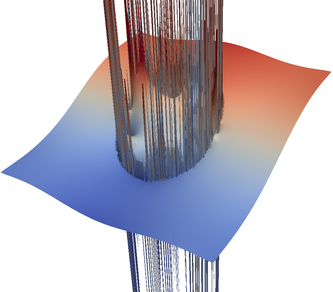
\includegraphics[width=0.14\textwidth]{q2q1/sinker-8-none.png}
    &
    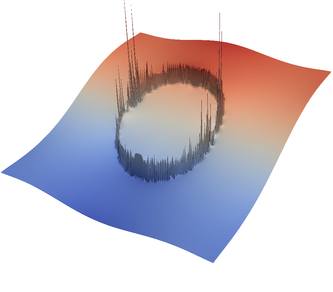
\includegraphics[width=0.14\textwidth]{q2q1/sinker-8-arithmetic.png}
    &
    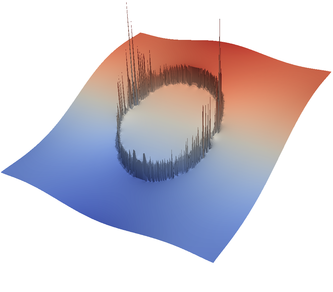
\includegraphics[width=0.14\textwidth]{q2q1/sinker-8-harmonic.png}
    &
    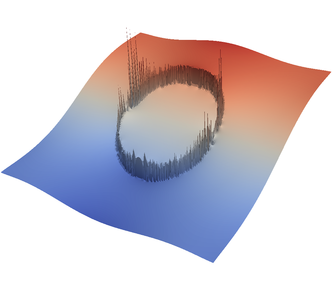
\includegraphics[width=0.14\textwidth]{q2q1/sinker-8-geometric.png}
    &
    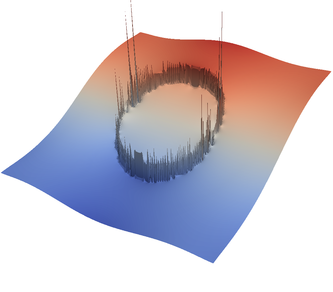
\includegraphics[width=0.14\textwidth]{q2q1/sinker-8-largest.png}
    &
    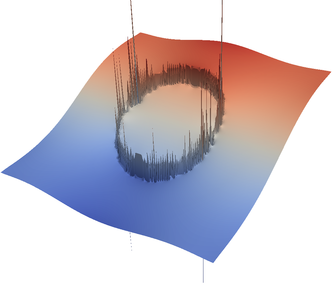
\includegraphics[width=0.14\textwidth]{q2q1/sinker-8-project.png}
    \\
    $[-44.5,44.5]$
    &
    $[-5.18,5.18]$
    &
    $[-5.09,5.09]$
    &
    $[-5.18,5.18]$
    &
    $[-5.20,5.20]$
    &
    $[-7.99,7.99]$
  \end{tabular}
  \caption{\it Visualization of the pressure field for the ``sinker''
    problem. Left to right: No averaging, arithmetic averaging, harmonic
    averaging, geometric averaging, pick largest, project to $Q_1$. Top: 7
    global refinement steps. Bottom: 8 global refinement steps. The minimal and maximal pressure
    values are indicated below every picture. This range is symmetric because
    we enforce that the average of the pressure equals zero. The color scale
    is adjusted to show only values between $p=-3$ and $p=3$.}
  \label{fig:sinker-with-averaging-pressure}
\end{figure}

\begin{table}[htb]
  \center
  \begin{tabular}{|c|cccccc|}
    \hline
    \# of global & no averaging & arithmetic & harmonic & geometric
    & pick & project \\
    refinement steps & & averaging & averaging &
    averaging & largest & to $Q_1$
    \\ \hline
    4          & 30+64   & 30+13      & 30+10    & 30+12 & 30+13 & 30+15 \\
    5          & 30+87   & 30+14      & 30+13    & 30+14 & 30+14 & 30+16 \\
    6          & 30+171  & 30+14      & 30+15    & 30+14 & 30+15 & 30+17 \\
    7          & 30+143  & 30+27      & 30+28    & 30+26 & 30+26 & 30+28 \\
    8          & 30+188  & 30+27      & 30+26    & 30+27 & 30+28 & 30+28 \\ \hline
  \end{tabular}
  \caption{\it Number of outer GMRES iterations to solve the Stokes equations
  for various numbers of global mesh refinement steps and for different
  material averaging operations. The GMRES solver first tries to run 30
  iterations with a cheaper preconditioner before switching to a more expensive
  preconditioner (see Section~\ref{parameters:Nonlinear solver tolerance}).}
  \label{tab:sinker-with-averaging-iteration-counts}
\end{table}
Such improvements carry over to more complex and realistic models. For
example, in a simulation of flow under the East African Rift by Sarah Stamps,
using approximately 17 million unknowns and run on 64 processors, the number
of outer and inner iterations is reduced from 169 and 114,482 without
averaging to 77 and 23,180 with harmonic averaging, respectively.
This translates into a reduction of run-time from 145 hours to 17
hours. Assessing the accuracy of the answers is of course more complicated in
such cases because we do not know the exact solution. However, the results
without and with averaging do not differ in any significant way.

A final comment is in order. First, one may think that the results should be
better in cases of discontinuous pressures if the numerical approximation
actually allowed for discontinuous pressures. This is in fact possible: We can
use a finite element in which the pressure space contains piecewise constants
(see Section~\ref{parameters:Discretization}). To do so, one simply needs to add
the following piece to the input file:
\lstinputlisting[language=prmfile]{conservative.prm.out}
Disappointingly, however, this makes no real difference: the pressure
oscillations are no better (maybe even worse) than for the standard Stokes
element we use, as shown in
Fig.~\ref{fig:sinker-with-averaging-pressure-q2q1iso} and
Table~\ref{tab:sinker-with-averaging-max-pressure-q2q1iso}. Furthermore, as
shown in Table~\ref{tab:sinker-with-averaging-iteration-counts-q2q1iso}, the
iteration numbers are also largely unaffected if any kind of averaging is used
-- though they are far worse using the locally conservative discretization if no
averaging has been selected. On the positive side, the visualization of the
discontinuous pressure finite element solution makes it much easier to see
that the true pressure is in fact discontinuous along the edge of the circle.

\begin{figure}[htb]
  \centering
  \begin{tabular}{cccccc}
    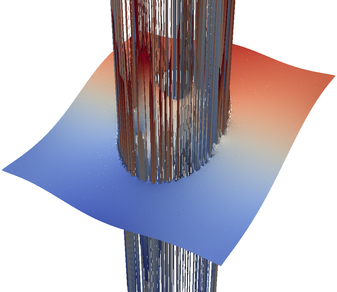
\includegraphics[width=0.14\textwidth]{q2q1plus/sinker-7-none.png}
    &
    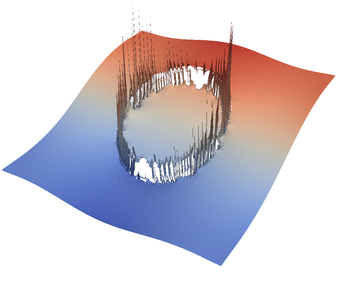
\includegraphics[width=0.14\textwidth]{q2q1plus/sinker-7-arithmetic.png}
    &
    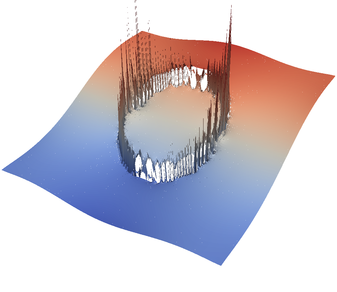
\includegraphics[width=0.14\textwidth]{q2q1plus/sinker-7-harmonic.png}
    &
    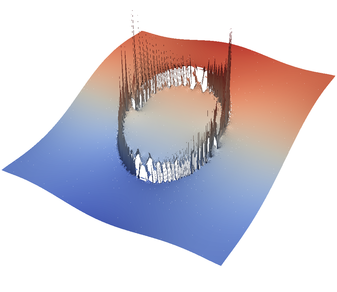
\includegraphics[width=0.14\textwidth]{q2q1plus/sinker-7-geometric.png}
    &
    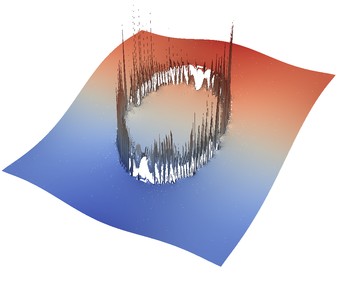
\includegraphics[width=0.14\textwidth]{q2q1plus/sinker-7-pick-largest.png}
    &
    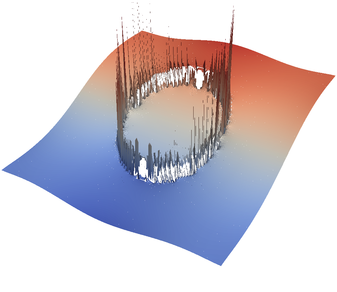
\includegraphics[width=0.14\textwidth]{q2q1plus/sinker-7-project-to-Q1.png}
    \\
    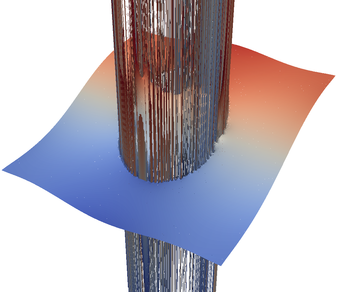
\includegraphics[width=0.14\textwidth]{q2q1plus/sinker-8-none.png}
    &
    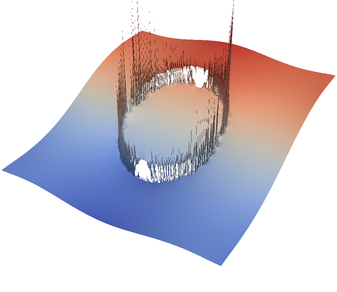
\includegraphics[width=0.14\textwidth]{q2q1plus/sinker-8-arithmetic.png}
    &
    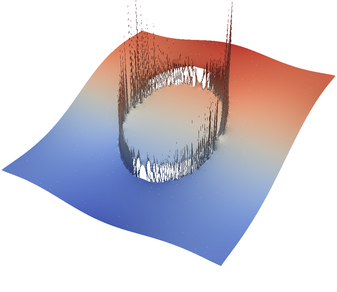
\includegraphics[width=0.14\textwidth]{q2q1plus/sinker-8-harmonic.png}
    &
    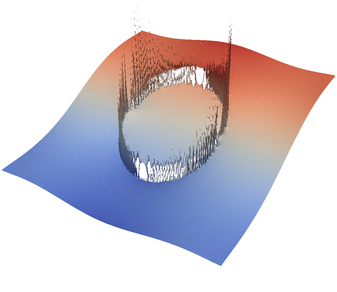
\includegraphics[width=0.14\textwidth]{q2q1plus/sinker-8-geometric.png}
    &
    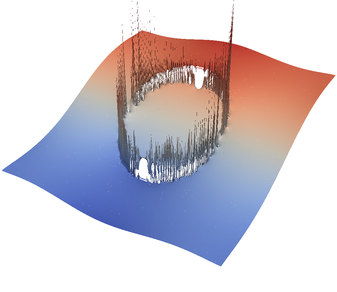
\includegraphics[width=0.14\textwidth]{q2q1plus/sinker-8-pick-largest.png}
    &
    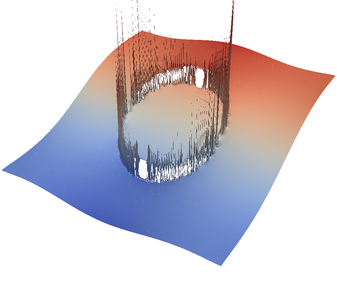
\includegraphics[width=0.14\textwidth]{q2q1plus/sinker-8-project-to-Q1.png}
  \end{tabular}
  \caption{\it Visualization of the pressure field for the ``sinker''
    problem. Like Fig.~\ref{fig:sinker-with-averaging-pressure} but using the
    locally conservative, enriched Stokes element. Pressure values are shown
    in Table~\ref{tab:sinker-with-averaging-max-pressure-q2q1iso}.}
  \label{fig:sinker-with-averaging-pressure-q2q1iso}
\end{figure}


\begin{table}[htb]
  \center
  \begin{tabular}{|c|cccccc|}
    \hline
    \# of global & no averaging & arithmetic & harmonic & geometric
    & pick & project \\
    refinement steps & & averaging & averaging &
    averaging & largest & to $Q_1$
    \\ \hline
    4 & 66.32 & 2.66 & 2.893 & 1.869 & 3.412 & 3.073 \\
    5 & 81.06 & 3.537 & 4.131 & 3.997 & 3.885 & 3.991 \\
    6 & 75.98 & 4.596 & 4.184 & 4.618 & 4.568 & 5.093 \\
    7 & 84.36 & 4.677 & 5.286 & 4.362 & 4.635 & 5.145 \\
    8 & 83.96 & 5.701 & 5.664 & 4.686 & 5.524 & 6.42 \\ \hline
  \end{tabular}
  \caption{\it Maximal pressure values for the ``sinker'' benchmark, using the
  locally conservative, enriched Stokes element. The corresponding
  pressure solutions are shown in
  Fig.~\ref{fig:sinker-with-averaging-pressure-q2q1iso}.}
  \label{tab:sinker-with-averaging-max-pressure-q2q1iso}
\end{table}


\begin{table}[htb]
  \center
  \begin{tabular}{|c|cccccc|}
    \hline
    \# of global & no averaging & arithmetic & harmonic & geometric
    & pick & project \\
    refinement steps & & averaging & averaging &
    averaging & largest & to $Q_1$
    \\ \hline
    4 & 30+376 & 30+16 & 30+12 & 30+14 & 30+14 & 30+17 \\
    5 & 30+484 & 30+16 & 30+14 & 30+14 & 30+14 & 30+16 \\
    6 & 30+583 & 30+16 & 30+17 & 30+14 & 30+17 & 30+17 \\
    7 & 30+1319 & 30+27 & 30+28 & 30+26 & 30+28 & 30+28 \\
    8 & 30+1507 & 30+28 & 30+27 & 30+28 & 30+28 & 30+29  \\ \hline
  \end{tabular}
  \caption{\it Like Table~\ref{tab:sinker-with-averaging-iteration-counts}, but
  using the locally conservative, enriched Stokes element.}
  \label{tab:sinker-with-averaging-iteration-counts-q2q1iso}
\end{table}


